\subsection{Overview of the UI}

A user interface (\emph{UI}) will help visualizing the game.
It will be coded in \emph{C++} and will use the graphic library \emph{SFML 1.6}.
Its funcionnalities will include the following:
\begin{itemize}
	\item 1 Versus 1, player versus AI and AI versus AI
	\item Mouse and keyboard controls
	\item Configurable controls and resolution
	\item Assisted unit placement
	\item Game saving and loading
	\item Game replay
	\item Fullscreen mode
	\item Graphical mods
\end{itemize}

\begin{figure}[!h]
\centering
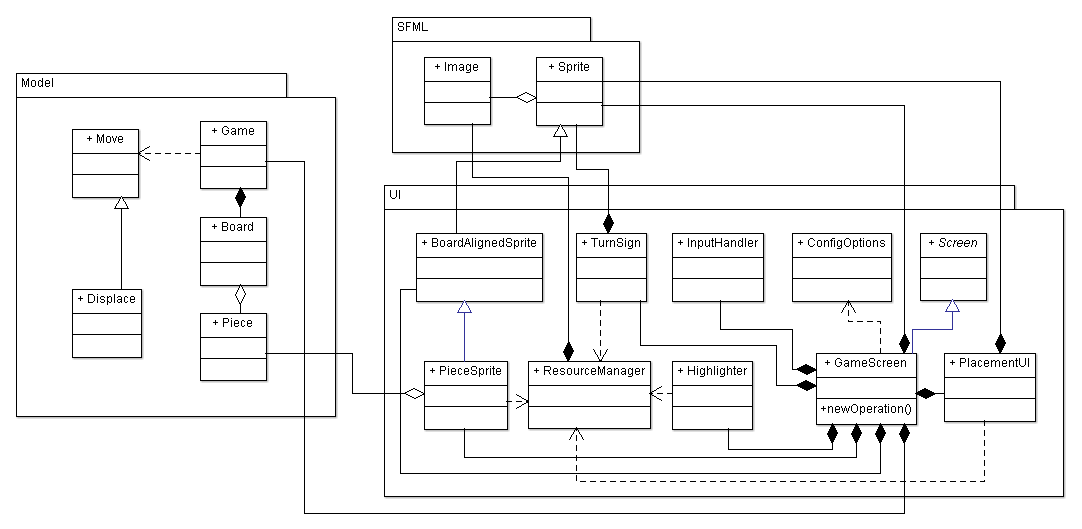
\includegraphics[width=\textwidth]{Gui/Img/Application_UML.png}
\caption{A UML diagram for the UI.}
\label{fig:UML_UI}
\end{figure}

A UML diagram for the UI is presented in figure \ref{fig:UML_UI}.
In this diagram, you can see three modules:
\begin{itemize}
	\item The model, rogrouping the rules of Arimaa
	\item The UI itself, handling the inputs and outputs, and interfacing with the Model
	\item The SFML, a library that loads and displays the assets
\end{itemize}

\subsection{The model}

The model handles the rules of the game.
A game is modelized by the class \emph{Game}.
This class conains a \emph{Board}, itself containing instances of \emph{Piece}.
While the \emph{Board} allows any and all modifications to the pieces' placement, the \emph{Game} only allows actions that follow the rules.
This is done through the use of the \emph{Move} class, representing a move in the game.
Any instance of the \emph{Move} class can be verified by the \emph{Game}, and executed if found valid.
The class \emph{Displace} inherits from \emph{Move}, and modelizes pushes and pulls.

\subsection{The UI}

The core of the UI lies in the class \emph{Screen}.
It modelizes a screen that can be displayed and updated at each frame.
The \emph{GameScreen} is the main screen of this UI : it displays the game as it is played.
Among the other important classes are \emph{ResourceManager}, that uses the \emph{Flyweight} design pattern to manage the assets;
then there is \emph{InputHandler}, that associates keyboard inputs with strings representing the different actions,
and also \emph{ConfigOptions}, that loads the options contained in a .ini file and relays them to the application.
Most of the other classes represent the different graphical elements (pieces, the cursor...) and will not be explained in detail here.